\section{Результаты}

Разработанное решение представляет собой программу на языке C, выполняющую многопоточную обработку матрицы вещественных чисел с применением фильтров эрозии и наращивания. Программа позволяет измерять время выполнения для различного числа потоков и строить график зависимости времени от количества потоков.
В результаты был получен графики зависимости времени от количества потоков и ускорения от количества потоков:

\begin{figure}[h]
    \centering
    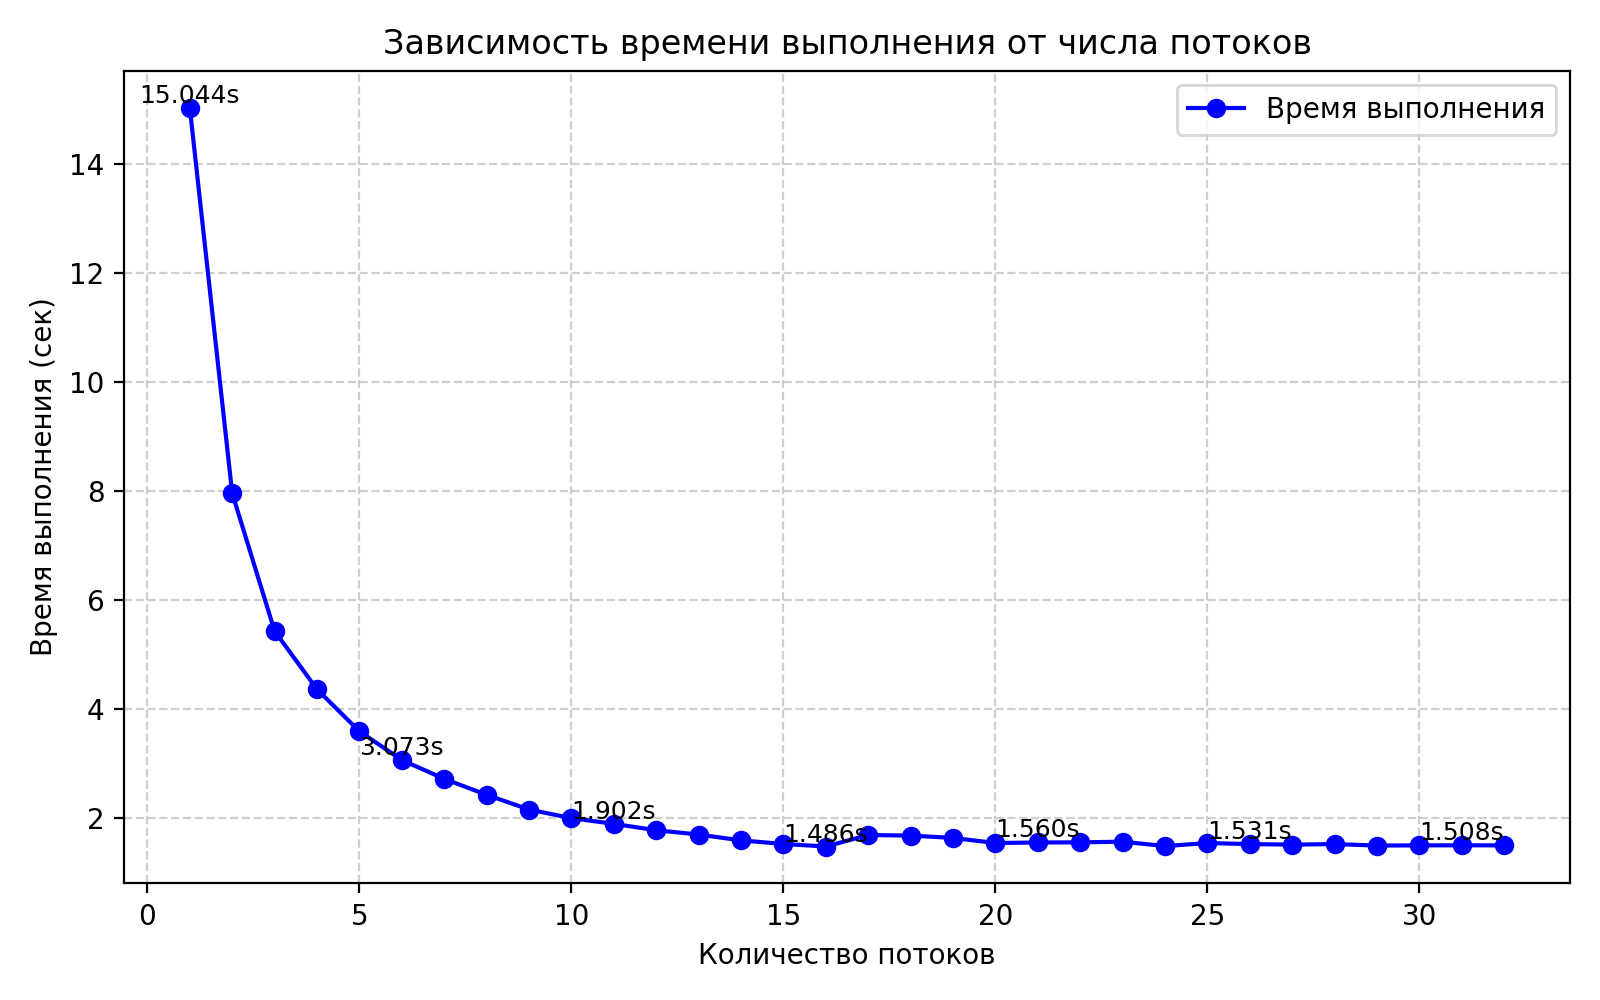
\includegraphics[width=0.75\textwidth]{src/results.png}
    \caption{График зависимости времени выполнения от количества используемых потоков.}
    \label{fig:graph}
\end{figure}

\begin{figure}[h]
    \centering
    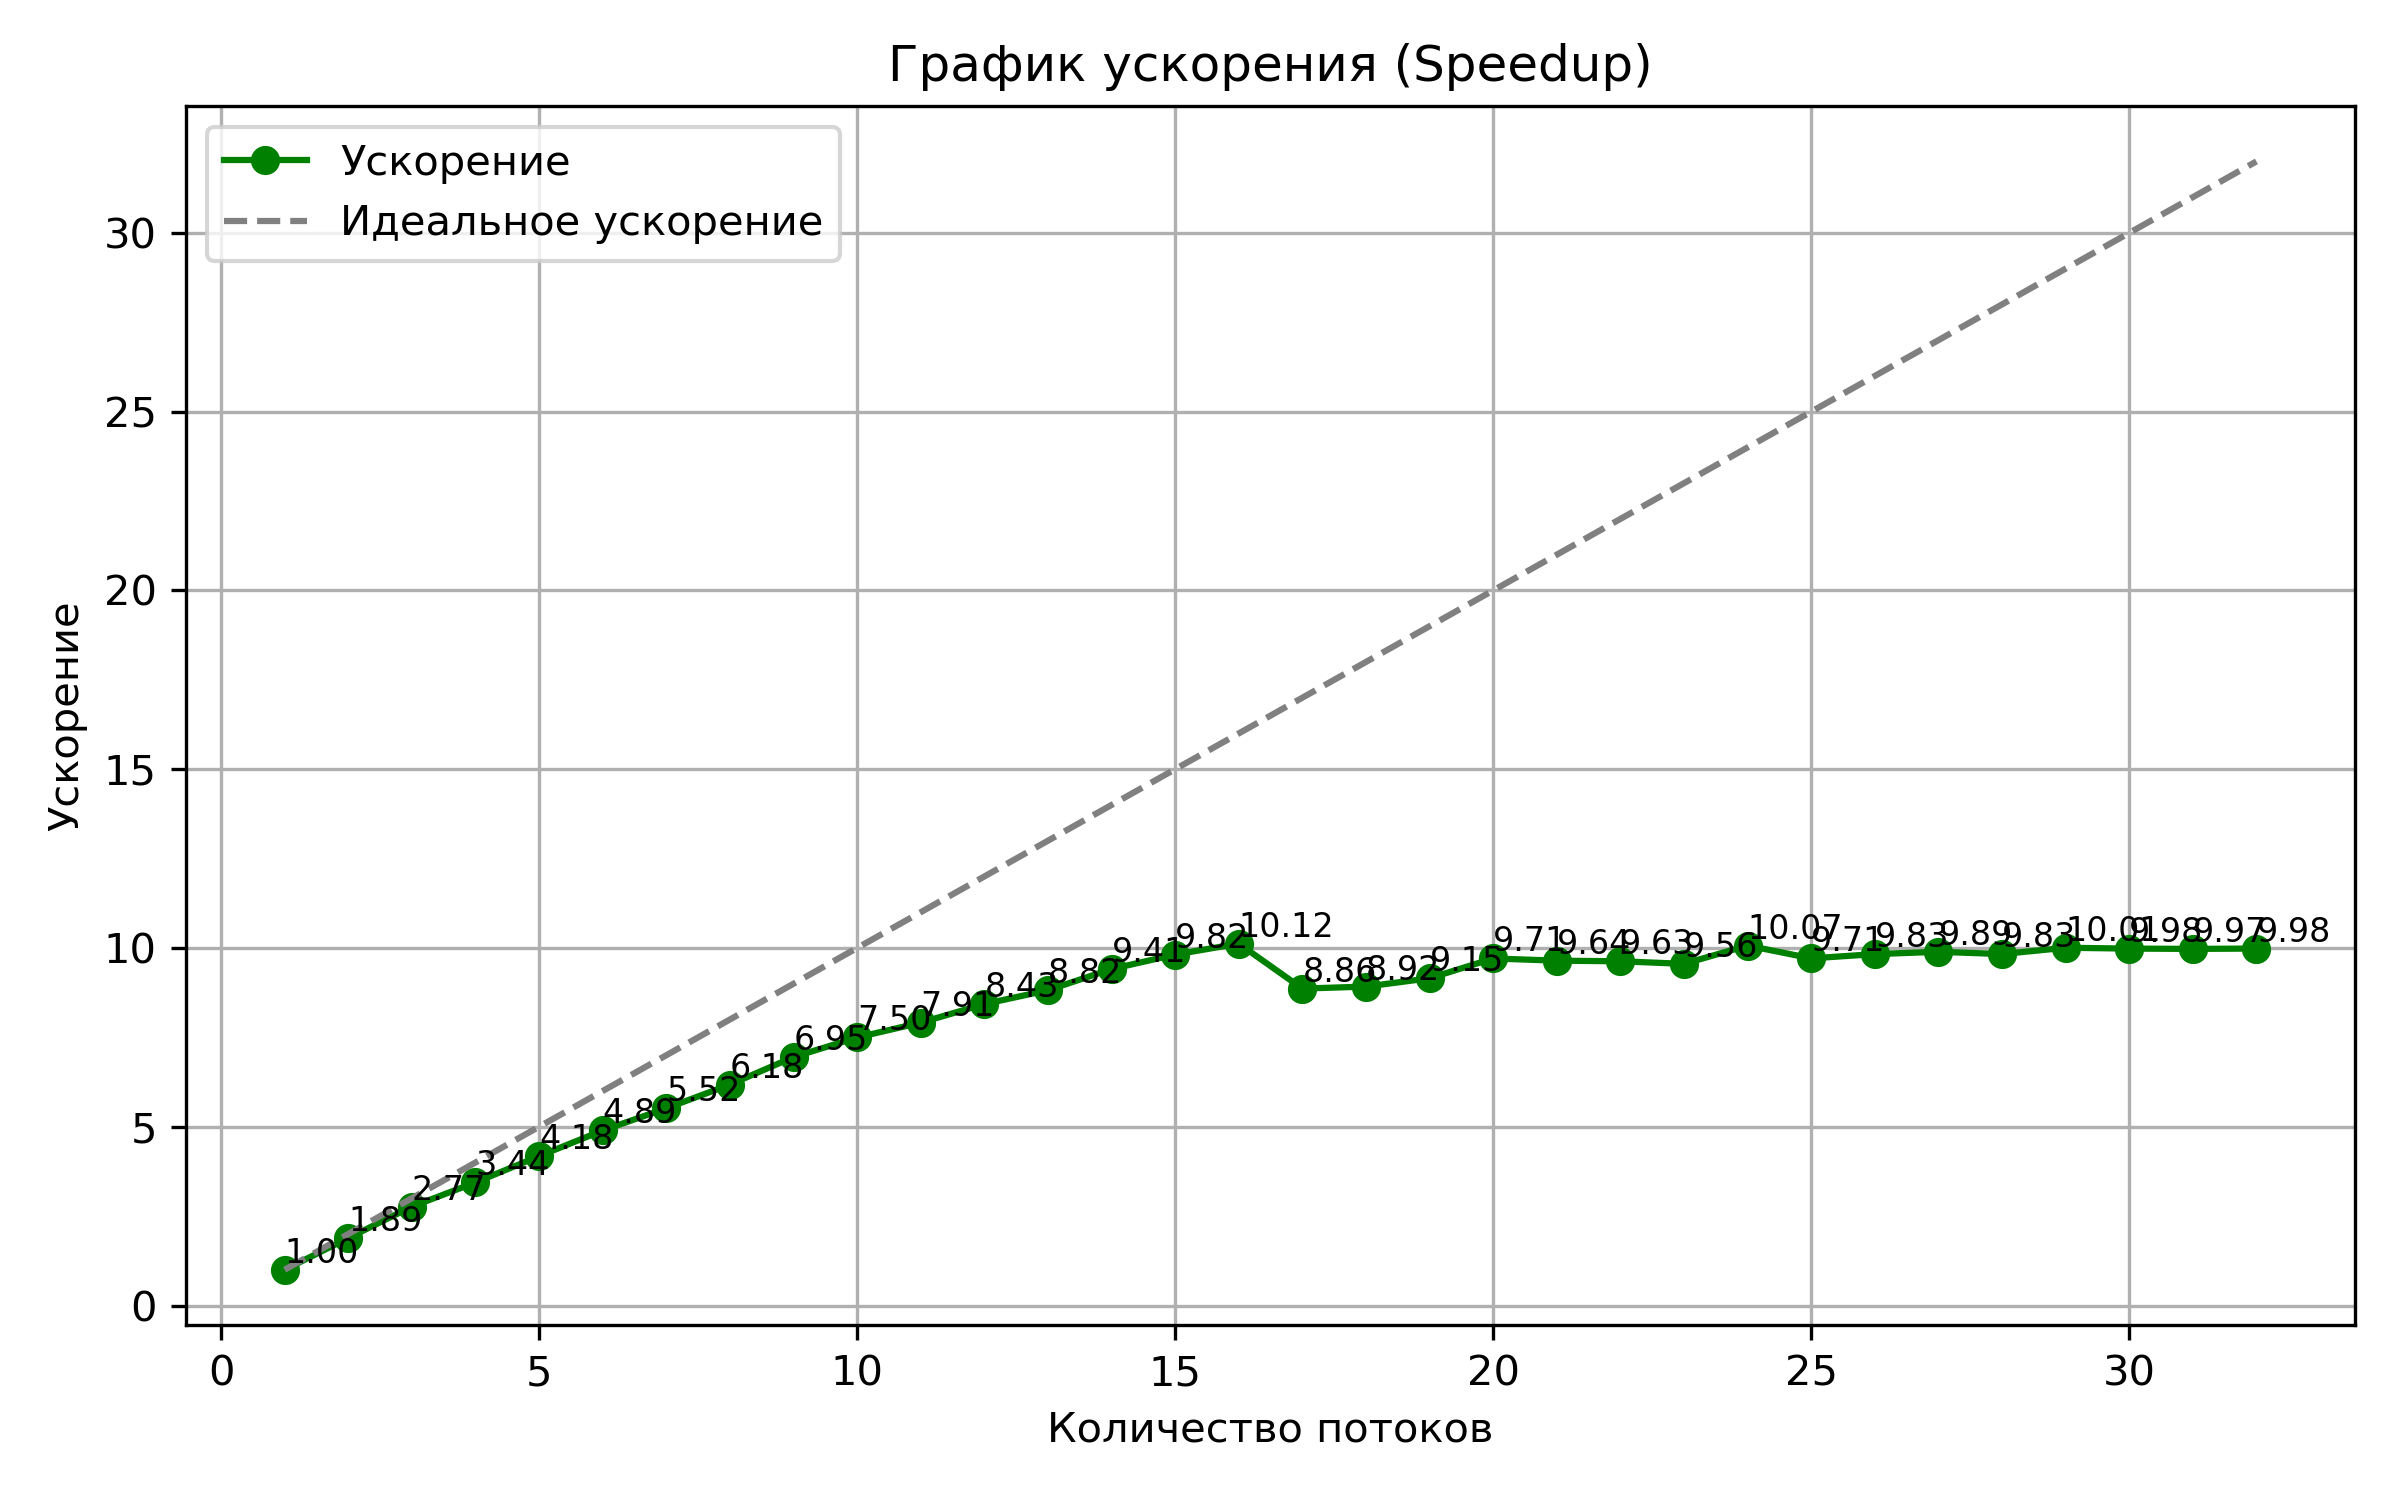
\includegraphics[width=0.75\textwidth]{src/results_speedup.png}
    \caption{График зависимости ускорения от количества используемых потоков.}
    \label{fig:graph}
\end{figure}

На представленных графиках показаны результаты экспериментального исследования производительности параллельной программы в зависимости от количества используемых потоков. 
Первый график иллюстрирует зависимость времени выполнения программы от числа потоков: при увеличении числа потоков с одного до примерно восьми–двенадцати время выполнения резко снижается, что свидетельствует о высокой эффективности распараллеливания на этом этапе; однако начиная с 16–20 потоков кривая выходит на плато — дальнейшее увеличение числа потоков практически не приводит к уменьшению времени выполнения, что обусловлено накладными расходами на управление потоками, ограниченной параллелизуемостью задачи по закону Амдала и аппаратными ограничениями процессора.
Второй график демонстрирует зависимость ускорения от числа потоков: реальное ускорение сначала близко к идеальному, но затем отклоняется от него, стабилизируясь на уровне около 10–11, что подтверждает наличие последовательной части программы и указывает на то, что дальнейшее увеличение числа потоков не даёт практической выгоды — оптимальное количество потоков для данной программы составляет 8–12, при котором достигается максимальная производительность без избыточной нагрузки на систему.

\subsection*{Ключевые особенности}
\begin{enumerate}
    \item Программа создаёт исходную матрицу размером $M \times N$ и два результирующих массива для эрозии и наращивания.
    \item Для повышения производительности используется многопоточность: работа распределяется между потоками статически по блокам строк.
    \item Максимальное количество потоков, работающих одновременно, задаётся пользователем через ключ запуска программы, что позволяет гибко контролировать нагрузку.
    \item Программа поддерживает многократное применение фильтров (K раз) на матрицу, обеспечивая возможность исследования разных сценариев нагрузки.
    \item Время выполнения каждого запуска сохраняется в CSV-файл \texttt{results.csv}, который затем используется для построения графика зависимости времени от числа потоков.
    \item Структура проекта разделена на папки \texttt{inc/} и \texttt{src/}, что облегчает поддержку и масштабирование кода.
\end{enumerate}
